\documentclass[journal]{IEEEtran}
%\usepackage{cite}
\usepackage{graphicx}
%\usepackage{circuitikz}
%\usepackage[cmex10]{amsmath}
%\usepackage{dblfloatfix}
%\usepackage{capt-of}
%\usepackage{breqn}
%\usepackage{listings}
%\usepackage{mathrsfs}
%\usepackage[scale=.8]{geometry}
%\usepackage{hyperref}
%\usepackage{breakurl}
\usepackage{epstopdf}
\usepackage[nomarkers,nolists,tablesfirst]{endfloat}
\renewcommand{\efloatseparator}{\mbox{}}

\begin{document}
% paper title
% can use linebreaks \\ within to get better formatting as desired
\title{A Switched-Capacitor Amplifier for Use in a 2.5bit/stage Pipelined Analog-to-Digital Converter }

\author{Joseph Meyer and Miles Sherman}

% The paper headers
\markboth{ELEN 6312 Advanced Analog Integrated Circuits}%
{Shell \MakeLowercase{\textit{et al.}}: Bare Demo of IEEEtran.cls for Journals}

\maketitle

\begin{abstract}
A switched-capacitor amplifier with a nominal gain of 4 was designed for use in a 2.5 bit/stage pipelined analog-to-digital converter (ADC). The total resolution of the ADC was 10 bits. The sample rate of the ADC was $5kS/s$. The amplifier consisted of 4 sample capacitors and 1 hold capacitor in feedback around an operational transconductance amplifier (OTA). The OTA consisted of a pMOS-input folded cascode stage followed by an nMOS common source stage. The open loop DC gain of the OTA was $110.9dB$. The unity gain bandwidth of the OTA was $87.1kHz$. The circuit consumed MAKE THIS MORE ACCURATE $725nW$ of DC power. SOMETHING ABOUT EFFECTIVE NUMBER OF BITS. SOMETHING ABOUT FIGURE OF MERIT.
\end{abstract}

% Note that keywords are not normally used for peerreview papers.
\begin{IEEEkeywords}
switched-capacitor amplifier, pipelined analog-to-digital converter
\end{IEEEkeywords}

\section{Introduction}
\IEEEPARstart {P}{ipelined} ADCs require accurate amplification in each stage for proper operation. The residue of each stage must be amplified to be properly processed by the subsequent stage. Pipelined ADCs implementing 2.5 bits per stage through comparator redundancy require a gain of 4. 

Switched-capacitor amplifiers are ideal for accurate amplifiers. Since the gain of switched-capacitor amplifiers relies only on ratios of capacitors (as opposed to ratios of multiple types component values), the gain of these amplifiers tends to be quite accurate.

\section{System Level Design}
\subsection{Top Level Schematic}
The schematic overall system level design is shown in Figure \ref{fig:system_level_schem}. With ideal switches and ideal OTA, this schematic yields an exact gain of 4. This section overviews the specifications for each of these components.

\begin{figure}
\centering
\includegraphics[width=5in]{Schematics/system_level_schem.png}
\caption{The system level schematic of the switched-capacitor amplifier.}
\label{fig:system_level_schem}
\end{figure}

\subsection{Common Mode Voltage}
We know that the common mode voltage at the input and output nodes should be the same for proper operation of the device. To maximize the voltage swing at the output, we must choose $V_{CM}$ to be exactly at mid-rail. Thus,
\begin{equation}
V_{cm}=\frac{V_{DD}}{2}=0.9V
\end{equation}

\subsection{Full Scale Voltage}
In our design, we can assume that the output of the OTA can swing between $V_{ov}$ and $V_{DD}-V_{ov}$. If we choose our $V_{FS}$ to occupy the entire swing at the output and make the assumption that $V_{ov}\approx 0.2V$, we find that
\begin{equation}
V_{FS} = \left(V_{DD} - V_{ov}\right) - V_{ov} = 1.4V
\end{equation}

\subsection{Least Significant Bit Voltage}
In our differential amplifier topology, the output can swing from $-V_{FS}$ to $V_{FS}$. Thus, we can calculate our least significant bit voltage as
\begin{equation}
V_{LSB}=\frac{2V_{FS}}{2^N}=2.73mV
\end{equation}

\subsection{Sample and Hold Capacitors}
We can find the minimum value of the hold and capacitor values from the noise requirements.


\subsection{Switches}

\section{Transistor Level OTA Design}
\subsection{Gain Stage}

\subsection{Biasing}

\subsection{Component Values}

\begin{table}
\centering
\caption{Passive Component Values}
\label{tab:passive_elements}
\begin{tabular}{|c|c|}
\hline Component & Value \\ 
\hline Resistors & $\Omega$ \\ 
\hline R0 & 40M \\ 
\hline R1 & 40M \\ 
\hline Capacitors & $fF$ \\ 
\hline $C_{comp}$ & 750 \\ 
\hline $C_{hold}$ & 150 \\ 
\hline $C_{samp}$ & 150 \\ 
\hline 
\end{tabular} 
\end{table}

\begin{table}
\centering
\caption{Transistor Sizings}
\label{tab:trans_sizes}
\begin{tabular}{|c|c|c|c|}
\hline Transistor & Width (nm) & Length (nm) & Aspect Ratio \\ 
\hline M1 & 300 & 8000 & 0.0375 \\ 
\hline M2 & 750 & 1000 & 0.75 \\ 
\hline M3 & 750 & 1000 & 0.75 \\ 
\hline M4a & 281 & 10000 & 0.0281 \\ 
\hline M4b & 281 & 10000 & 0.0281 \\ 
\hline M4c & 281 & 10000 & 0.0281 \\ 
\hline M5a & 281 & 10000 & 0.0281 \\ 
\hline M5b & 281 & 10000 & 0.0281 \\
\hline M5c & 281 & 10000 & 0.0281  \\
\hline M6 & 250 & 1330 & 0.188 \\
\hline M7 & 250 & 1330 & 0.188 \\
\hline M8 & 750 & 1000 & 0.75 \\
\hline M9 & 750 & 1000 & 0.75 \\
\hline M10a & 281 & 7500 & 0.0375 \\
\hline M10b & 281 & 7500 & 0.0375 \\
\hline M11a & 281 & 7500 & 0.0375  \\
\hline M11b & 281 & 7500 & 0.0375 \\
\hline M12 & 500 & 1000 & 0.5 \\
\hline M13 & 500 & 1000 & 0.5  \\
\hline M14 & 300 & 4000 & 0.075 \\
\hline M15 & 300 & 4000 & 0.075  \\
\hline M16 & 250 & 4000 & 0.0625 \\
\hline M17 & 250 & 4000 & 0.0625  \\
\hline M18a & 250 & 6800 & 0.0368 \\
\hline M18b & 250 & 6800 & 0.0368  \\
\hline M19a & 250 & 6800 & 0.0368 \\
\hline M19b & 250 & 6800 & 0.0368 \\
\hline M20a & 281 & 10000 & 0.0281 \\
\hline M20b & 281 & 10000 & 0.0281  \\
\hline M20c & 281 & 10000 & 0.0281  \\
\hline M21 & 750 & 1000 & 0.75 \\
\hline M22a & 300 & 8000 & 0.0375 \\
\hline M22b & 300 & 8000 & 0.0375 \\
\hline M23 & 300 & 8000 & 0.0375 \\
\hline M24 & 1500 & 1000 & 1.5 \\
\hline M25a & 250 & 10000 & 0.025 \\
\hline M25b & 250 & 10000 & 0.025  \\
\hline M25c & 250 & 10000 & 0.025 \\
\hline M25d & 250 & 10000 & 0.025 \\
\hline M25e & 250 & 10000 & 0.025 \\
\hline M25f & 250 & 10000 & 0.025 \\
\hline M26 & 750 & 1000 & 0.75 \\
\hline M27a & 300 & 8000 & 0.0375 \\
\hline M27b & 300 & 8000 & 0.0375  \\
\hline M28 & 250 & 1330 & 0.188 \\
\hline M29a & 281 & 10000 & 0.0281 \\
\hline M29b & 281 & 10000 & 0.0281  \\
\hline M29c & 281 & 10000 & 0.0281 \\
\hline M29d & 281 & 10000 & 0.0281 \\
\hline M29e & 281 & 10000 & 0.0281 \\
\hline M29f & 281 & 10000 & 0.0281 \\
\hline M30 & 750 & 1000 & 0.75 \\
\hline M31a & 300 & 8000 & 0.0375 \\
\hline M31b & 300 & 8000 & 0.0375  \\
\hline M32a & 250 & 7500 & 0.0333  \\
\hline M33a & 281 & 10000 & 0.0281 \\
\hline M33b & 281 & 10000 & 0.0281   \\
\hline M33c & 281 & 10000 & 0.0281   \\
\hline M33d & 281 & 10000 & 0.0281   \\
\hline M33e & 281 & 10000 & 0.0281   \\
\hline M33f & 281 & 10000 & 0.0281  \\
\hline M34a & 250 & 7330 & 0.0341 \\
\hline M34b & 250 & 7330 & 0.0341  \\
\hline M34c & 250 & 7330 & 0.0341  \\
\hline M35a & 250 & 7500 & 0.0333 \\
\hline M35b & 250 & 7500 & 0.0333  \\
\hline M36a & 281 & 10000 & 0.0281 \\
\hline M36b & 281 & 10000 & 0.0281 \\
\hline M36c & 281 & 10000 & 0.0281 \\
\hline M36d & 281 & 10000 & 0.0281 \\
\hline M36e & 281 & 10000 & 0.0281 \\
\hline M36f & 281 & 10000 & 0.0281 \\
\hline M37 & 300 & 4000 & 0.075 \\
\hline M38 & 281 & 3750 & 0.0749 \\
\hline M39a & 281 & 7500 & 0.0375 \\
\hline M39b & 281 & 7500 & 0.0375 \\
\hline 
\end{tabular} 
\end{table}

\section{Open Loop OTA Results}
\subsection{Common Mode Feedback Frequency Response}

\subsection{Open Loop Differential Frequency Response}
Open Loop Differential Magnitude Response

\begin{figure}
\centering
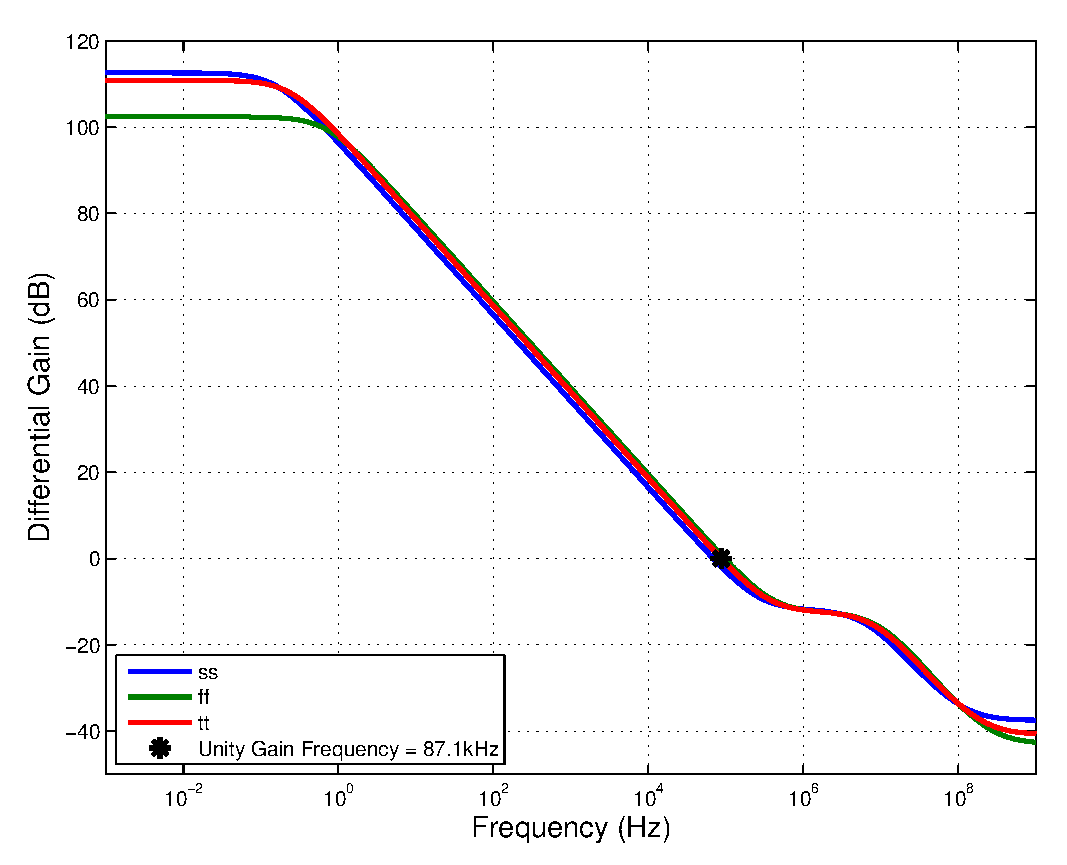
\includegraphics[width=4in]{Plots/open_dm_gain.eps}
\caption{The open loop differential gain magnitude response of the OTA.}
\label{fig:open_dm_gain}
\end{figure}


Open Loop Differential Phase Responses
\begin{figure}
\centering
\includegraphics[width=4in]{Plots/open_dm_phase.eps}
\caption{The open loop differential gain phase response of the OTA.}
\label{fig:open_dm_phase}
\end{figure}

\subsection{Open Loop Common Frequency Mode Response}

Open Loop Common Mode Magnitude Response
\begin{figure}
\centering
\includegraphics[width=4in]{Plots/open_cm_gain.eps}
\caption{The open loop common mode gain magnitude response of the OTA.}
\label{fig:open_cm_gain}
\end{figure}

Open Loop Common Mode Phase Response
\begin{figure}
\centering
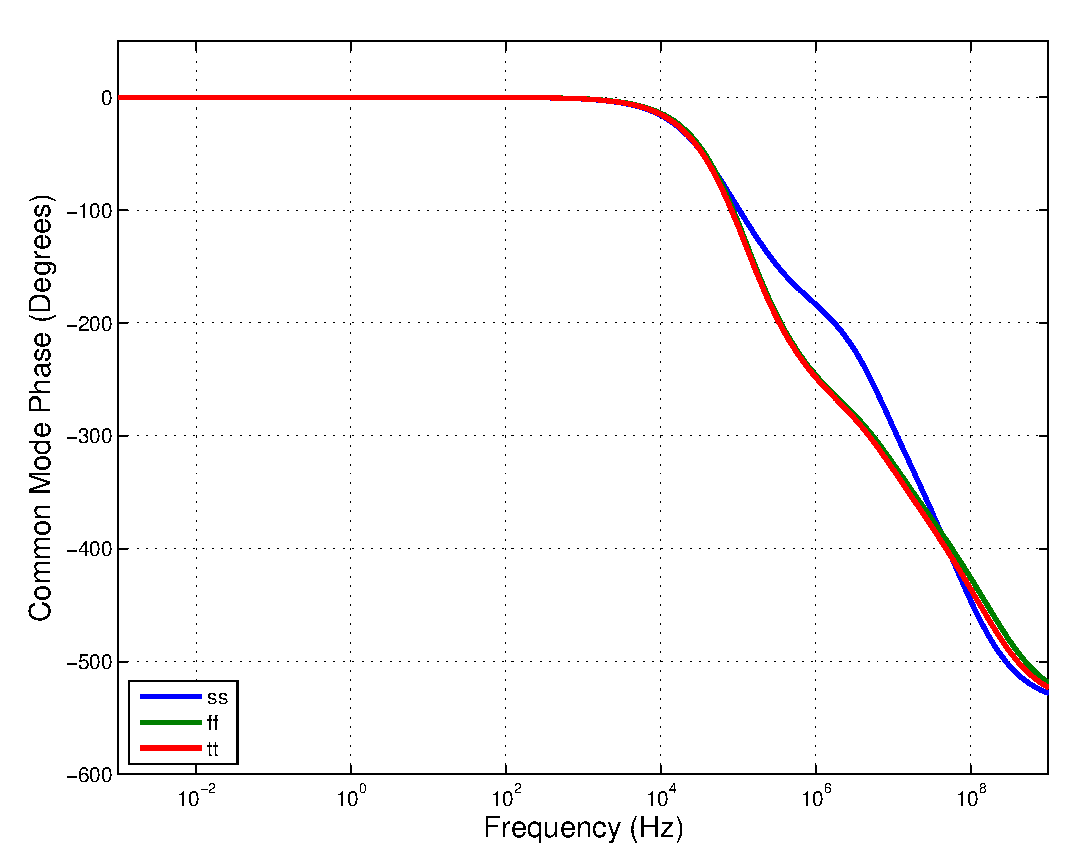
\includegraphics[width=4in]{Plots/open_cm_phase.eps}
\caption{The open loop common mode gain phase response of the OTA.}
\label{fig:open_cm_phase}
\end{figure}

\section{Closed Loop Amplifier Results}

\subsection{Nyquist Rate Sinusoidal Transient Response}

\begin{figure}
\centering
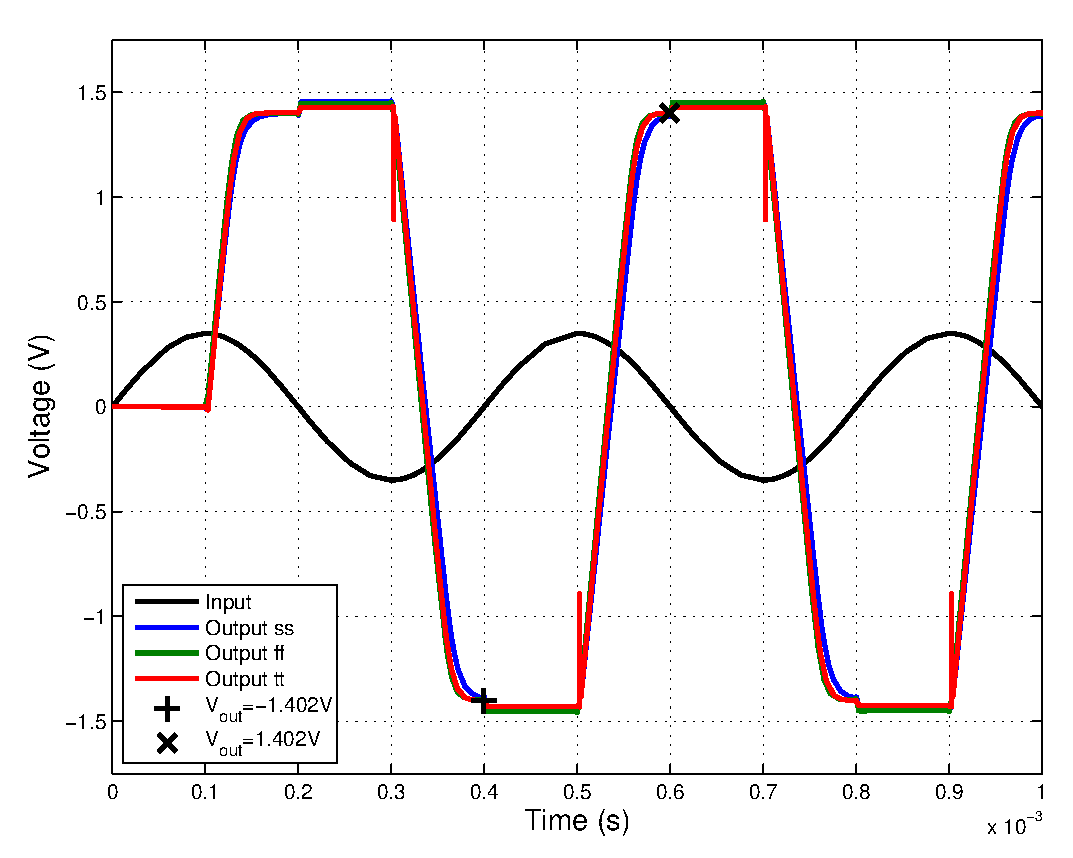
\includegraphics[width=4in]{Plots/closed_sine.eps}
\caption{The closed loop transient response to a full-scale amplitude sinusoid at the Nyquist frequency.}
\label{fig:closed_sine}
\end{figure}


\subsection{Small Step Transient Response}
\begin{figure}
\centering
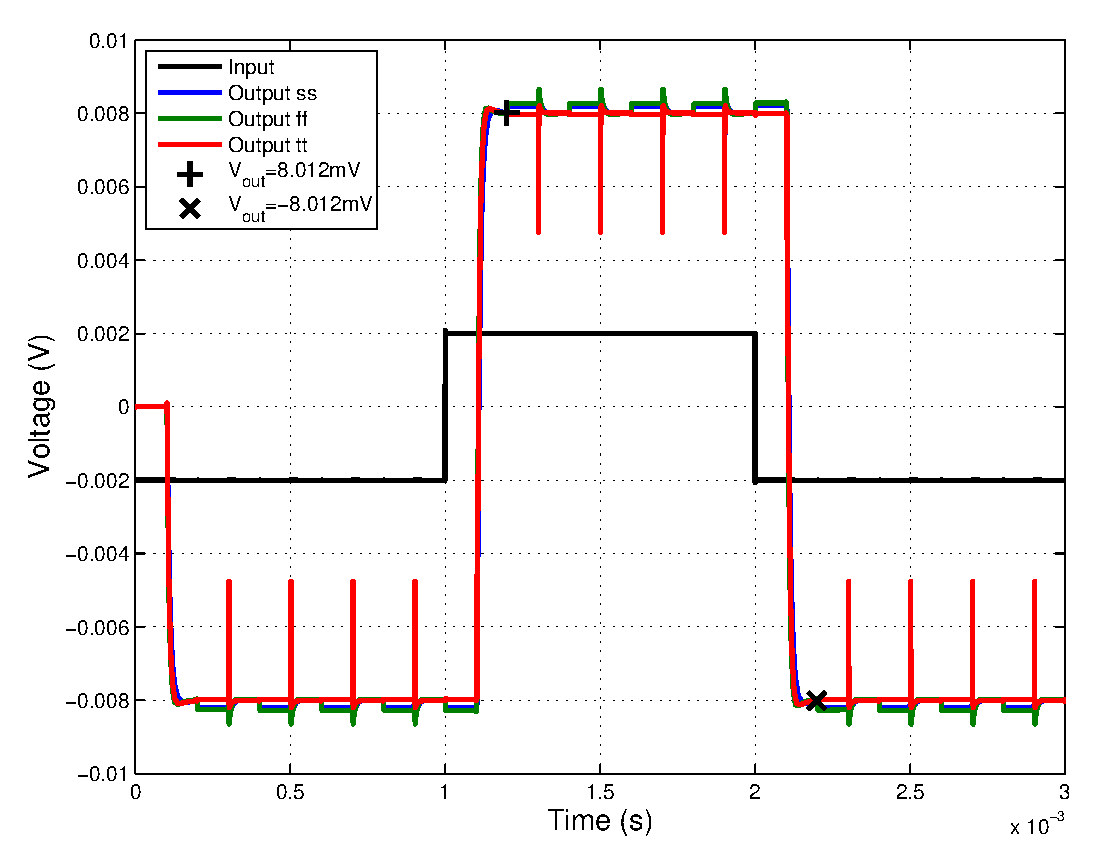
\includegraphics[width=4in]{Plots/closed_small_step.eps}
\caption{The closed loop transient response to a small amplitude step input.}
\label{fig:closed_small_step}
\end{figure}


\subsection{Full Scale Step Transient Response}
\begin{figure}
\centering
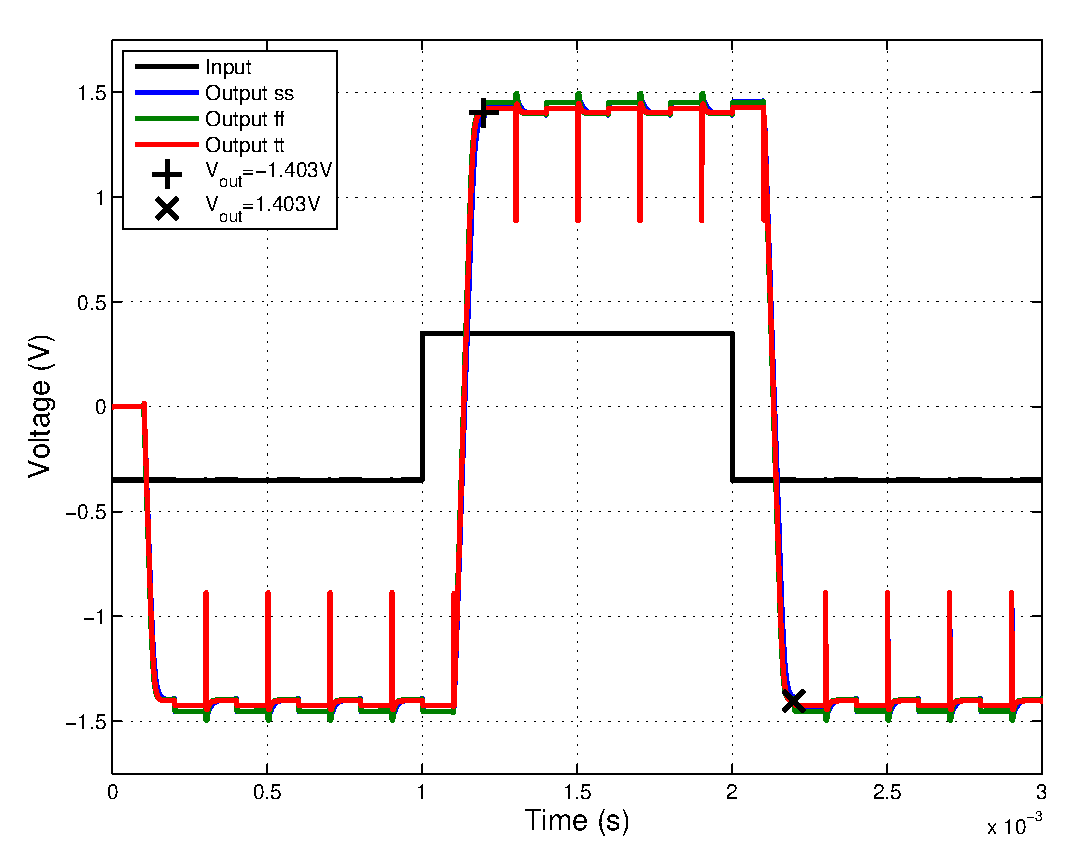
\includegraphics[width=4in]{Plots/closed_large_step.eps}
\caption{The closed loop transient response to a full-scale amplitude step input.}
\label{fig:closed_large_step}
\end{figure}

\subsection{Sawtooth Transient Response}
\begin{figure}
\centering
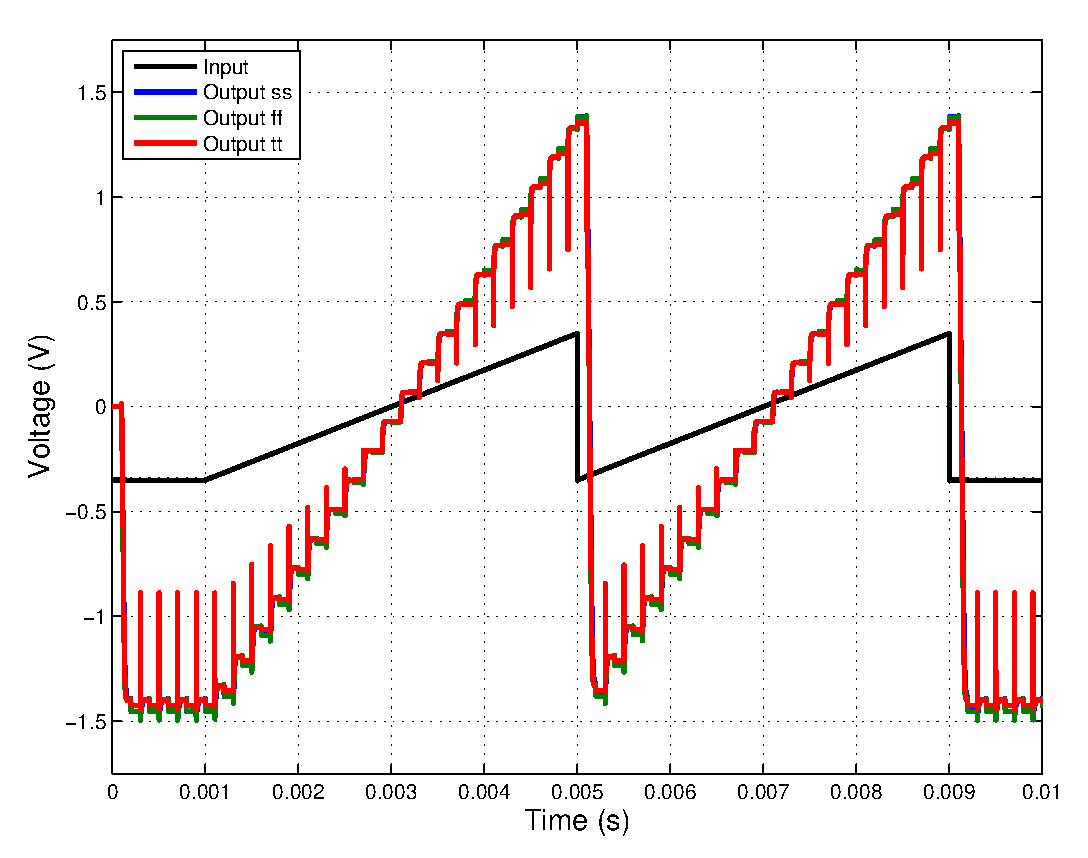
\includegraphics[width=4in]{Plots/closed_saw.eps}
\caption{The closed loop transient response to a full-scale amplitude sawtooth with a frequency of $\frac{f_s}{20}$.}
\label{fig:closed_saw}
\end{figure}

\subsection{Effective Number of Bits}

\subsection{Figure of Merit}

\subsection{Area}
transistor area

resistor area

capacitor area

total area

\section{Summary of Results}

\begin{table}
\centering
\caption{Summary of Specifications and Results}
\label{tab:specs_results}
\begin{tabular}{|c|c|c|c|c|}
\hline Specification & Specification Value & FF Result & TT Result & SS Result\\ 
\hline Open Loop OTA DC Gain &  & &  & \\ 
\hline Open Loop OTA Phase Margin &  & &  & \\ 
\hline Open Loop OTA $3dB$ Bandwidth &  & &  & \\ 
\hline Open Loop OTA Unity Gain Bandwidth &  & &  & \\ 
\hline Overall Power Consumption &  & &  & \\ 
\hline Overall Figure of Merit &  & &  & \\ 
\hline Overall Area &  & &  & \\ 
\hline  &  & &  & \\ 
\hline 
\end{tabular} 
\end{table}


\section{Possible Improvements}

\section{Conclusion}


% references section

% can use a bibliography generated by BibTeX as a .bbl file
% BibTeX documentation can be easily obtained at:
% http://www.ctan.org/tex-archive/biblio/bibtex/contrib/doc/
% The IEEEtran BibTeX style support page is at:
% http://www.michaelshell.org/tex/ieeetran/bibtex/
%\bibliographystyle{IEEEtran}
% argument is your BibTeX string definitions and bibliography database(s)
%\bibliography{IEEEabrv,../bib/paper}
%
% <OR> manually copy in the resultant .bbl file
% set second argument of \begin to the number of references
% (used to reserve space for the reference number labels box)
%%\begin{thebibliography}{1}
%%
%%\bibitem{sedrasmith}
%%A.~Sedra and K.~Smith, \emph{Microelectronic Circuits}, 6th~ed. \\ 
%%Oxford University Group, 2009. pgs. 711-716.  
%%\bibitem{LowGroupDelay}
%%Kim, J.; Buckwalter, J.F.; "Bandwidth Enhancement With Low Group-Delay Variation for a 40-Gb/s Transimpedance Amplifier," \emph{Circuits and Systems I: Regular Papers, IEEE Transactions on} , vol.57, no.8, pp.1964-1972, Aug. 2010.
%%
%%\end{thebibliography}

%\bibliographystyle{plain}
%\bibliography{AnalogProjectReferences}

\end{document}